\subsection{Interactions}\label{HiC:interactions}% __14a-interactions
%~~~~~~~~~~~~~~~~~~~%
\subsubsection{Input} % inputs
Data from the pipeline \texttt{matrix-filtered} step is used as input (Section~\ref{HiC:matrix-filtered}).
%~~~~~~~~~~~~~~~~~~~%
\subsubsection{Analysis} % analysis
Default parameters:
\begin{lstlisting}
#!/bin/tcsh

source ./inputs/params/params.tcsh

set chrom_excluded = 'chr[MYX]'       # excluded chromosomes

set loop_params = "--bin-size=$bin_size --lambda-id=6 --rpk2b-cutoff=1.0 --loop-cutoff=4.0 --min-distance=40000"        # parameters for identifying significant interactions
\end{lstlisting}

%~~~~~~~~~~~~~~~~~~~%
\subsubsection{Output} % outputs
See Figure~\ref{fig:interactions_plots}. Default output:
\begin{lstlisting}
drwxr-xr-x  2 at570 3.3K Feb  5 10:12 __jdata
-rw-r--r--  1 at570 4.8K Feb  5 10:17 job.err
-rw-r--r--  1 at570   47 Feb  5 10:11 job.id
-rw-r--r--  1 at570    0 Feb  5 10:11 job.out
-rw-r--r--  1 at570  375 Feb  5 10:11 job.sh
-rw-r--r--  1 at570 3.6K Feb  5 10:17 job.vars.tsv
drwxr-xr-x  2 at570   54 Feb  5 10:15 matrix.chr1
drwxr-xr-x  2 at570   54 Feb  5 10:14 matrix.chr10
drwxr-xr-x  2 at570   54 Feb  5 10:14 matrix.chr11
drwxr-xr-x  2 at570   54 Feb  5 10:14 matrix.chr12
drwxr-xr-x  2 at570   54 Feb  5 10:13 matrix.chr13
drwxr-xr-x  2 at570   54 Feb  5 10:13 matrix.chr14
drwxr-xr-x  2 at570   54 Feb  5 10:13 matrix.chr15
drwxr-xr-x  2 at570   54 Feb  5 10:13 matrix.chr16
drwxr-xr-x  2 at570   54 Feb  5 10:13 matrix.chr17
drwxr-xr-x  2 at570   54 Feb  5 10:13 matrix.chr18
drwxr-xr-x  2 at570   54 Feb  5 10:13 matrix.chr19
drwxr-xr-x  2 at570   54 Feb  5 10:16 matrix.chr2
drwxr-xr-x  2 at570   54 Feb  5 10:13 matrix.chr20
drwxr-xr-x  2 at570   54 Feb  5 10:12 matrix.chr21
drwxr-xr-x  2 at570   54 Feb  5 10:13 matrix.chr22
drwxr-xr-x  2 at570   54 Feb  5 10:15 matrix.chr3
drwxr-xr-x  2 at570   54 Feb  5 10:15 matrix.chr4
drwxr-xr-x  2 at570   54 Feb  5 10:15 matrix.chr5
drwxr-xr-x  2 at570   54 Feb  5 10:15 matrix.chr6
drwxr-xr-x  2 at570   54 Feb  5 10:14 matrix.chr7
drwxr-xr-x  2 at570   54 Feb  5 10:14 matrix.chr8
drwxr-xr-x  2 at570   54 Feb  5 10:14 matrix.chr9
\end{lstlisting}

\begin{lstlisting}
matrix.chr1$
-rw-r--r--  1 at570 4.7M Feb  5 10:15 loops.tsv
-rw-r--r--  1 at570  27K Feb  5 10:16 plots.pdf
\end{lstlisting}
% ~/projects/hic-manual-report/report-base/figure/interactions_plots.pdf
\begin{figure}[!htb]
    \centering
    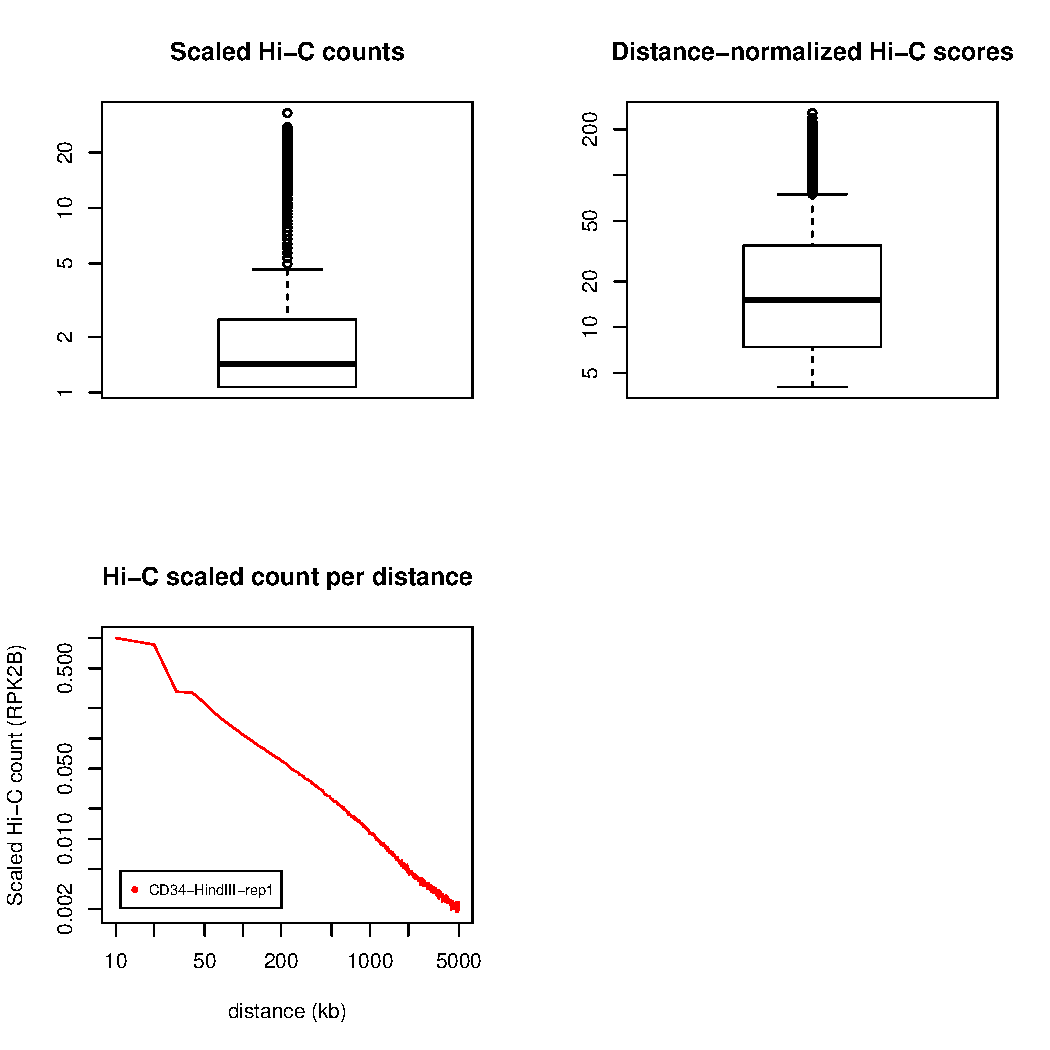
\includegraphics[width=\textwidth,height=\textheight,keepaspectratio]{figure/interactions_plots}
    \caption{Interactions sample output} % results/interactions.by_sample.standard/matrix-filtered.by_sample.res_10kb.maxd_5Mb.rotate45/filter.by_sample.standard/align.by_sample.bowtie2/CD34-HindIII-rep1/matrix.chr1
    \label{fig:interactions_plots}
\end{figure}
% \newpage
\clearpage